\documentclass{article}\usepackage[]{graphicx}\usepackage[]{xcolor}
% maxwidth is the original width if it is less than linewidth
% otherwise use linewidth (to make sure the graphics do not exceed the margin)
\makeatletter
\def\maxwidth{ %
  \ifdim\Gin@nat@width>\linewidth
    \linewidth
  \else
    \Gin@nat@width
  \fi
}
\makeatother

\definecolor{fgcolor}{rgb}{0.345, 0.345, 0.345}
\newcommand{\hlnum}[1]{\textcolor[rgb]{0.686,0.059,0.569}{#1}}%
\newcommand{\hlstr}[1]{\textcolor[rgb]{0.192,0.494,0.8}{#1}}%
\newcommand{\hlcom}[1]{\textcolor[rgb]{0.678,0.584,0.686}{\textit{#1}}}%
\newcommand{\hlopt}[1]{\textcolor[rgb]{0,0,0}{#1}}%
\newcommand{\hlstd}[1]{\textcolor[rgb]{0.345,0.345,0.345}{#1}}%
\newcommand{\hlkwa}[1]{\textcolor[rgb]{0.161,0.373,0.58}{\textbf{#1}}}%
\newcommand{\hlkwb}[1]{\textcolor[rgb]{0.69,0.353,0.396}{#1}}%
\newcommand{\hlkwc}[1]{\textcolor[rgb]{0.333,0.667,0.333}{#1}}%
\newcommand{\hlkwd}[1]{\textcolor[rgb]{0.737,0.353,0.396}{\textbf{#1}}}%
\let\hlipl\hlkwb

\usepackage{framed}
\makeatletter
\newenvironment{kframe}{%
 \def\at@end@of@kframe{}%
 \ifinner\ifhmode%
  \def\at@end@of@kframe{\end{minipage}}%
  \begin{minipage}{\columnwidth}%
 \fi\fi%
 \def\FrameCommand##1{\hskip\@totalleftmargin \hskip-\fboxsep
 \colorbox{shadecolor}{##1}\hskip-\fboxsep
     % There is no \\@totalrightmargin, so:
     \hskip-\linewidth \hskip-\@totalleftmargin \hskip\columnwidth}%
 \MakeFramed {\advance\hsize-\width
   \@totalleftmargin\z@ \linewidth\hsize
   \@setminipage}}%
 {\par\unskip\endMakeFramed%
 \at@end@of@kframe}
\makeatother

\definecolor{shadecolor}{rgb}{.97, .97, .97}
\definecolor{messagecolor}{rgb}{0, 0, 0}
\definecolor{warningcolor}{rgb}{1, 0, 1}
\definecolor{errorcolor}{rgb}{1, 0, 0}
\newenvironment{knitrout}{}{} % an empty environment to be redefined in TeX

\usepackage{alltt}
\title{\textbf{Discussion Assignment 2}}
\author{\textbf{Katherine Wolf}\\ Introduction to Causal Inference (PH252D)\\ \today}
\date{}

% list of latex packages you'll need
\usepackage{float}  % for tables
\usepackage{mathtools}  % for mathematical symbols
\usepackage{bm}  % to bold mathematical symbols like betas
\usepackage{scrextend}  % to indent subsections
\usepackage{xltxtra}
\usepackage{fontspec}
\usepackage{xunicode}
\usepackage[skip=0.5\baselineskip]{caption}  % control caption printing space
\usepackage{longtable}
\usepackage{amsmath}
\usepackage{amsfonts}
\usepackage{bm}
\usepackage{caption}
\usepackage[shortlabels]{enumitem}
\usepackage{txfonts}
\usepackage{dejavu}

% set fonts
\setmainfont{Georgia}
\setsansfont[Scale=MatchLowercase]{Arial}  % sets the sans font
\setmonofont[Scale=MatchLowercase]{DejaVuSansMono}  % sets the monospace font

% make special code formatting
\NewDocumentCommand{\codeword}{v}{%
  \texttt{{#1}}%
}

% set the margins of the document
\usepackage[top=1in, bottom=1in, left=.5in, right=.5in]{geometry}
\setlength\parindent{0pt}



% end the preamble and begin the document
\IfFileExists{upquote.sty}{\usepackage{upquote}}{}
\begin{document}

\maketitle

\section{Instructions}

\section{Background}

\section{Questions to be answered}

\setlength{\leftskip}{0.8cm}

\begin{enumerate}[label=\textbf{\arabic*.}]

  \item \textbf{Specify your observed data.}
  
  \begin{enumerate}[label=\textbf{(\alph*)}]
  
    \item \textbf{What notation do we use to refer to the distribution of the observed data?}
    
    $\mathbb{P}_{\bm{O}}$, as in $\bm{O} = (\bm{W}, \bm{A}, \bm{Y}) \sim \mathbb{P}_{\bm{O}}.$
  
    \item \textbf{Specify the link between the SCM and the observed data.}
    
We link the the observed data to the SCM by assuming that we obtained the observed data $\bm{O}$ from some data-generating system compatible with our SCM $\mathcal{M}^\mathcal{F}$, i.e., that each observation in the data represents a draw $\bm{U} = \bm{u}$ from the unknown probability distribution $\mathbb{P}_{\bm{U}}$ of the exogenous variables $\bm{U}$, which we then plugged into our structural equations $\mathcal{F}$ to output a specific $\bm{X} = \bm{x}$, of which we observed the subset $\bm{O} = \bm{o}$.
    
Thus we assume that applying the structural equations $\mathcal{F}$ to $\bm{U} \sim \mathbb{P}_{\bm{U}}$ will identify the distribution $\bm{X} \sim \mathbb{P}_{\bm{X}}$ and, since $\bm{O} \subseteq \bm{X}$, the distribution of its observed subset $\bm{O} \sim \mathbb{P}_{\bm{O}}$. (Since here we assume that $\bm{X} = \bm{O}$, we can write $P_{\bm{O}}(\bm{O} = \bm{o}) = \sum\limits_{\bm{u}}P_f(\bm{X}=\bm{x}|\bm{U}=\bm{u})P(\bm{U}=\bm{u}) = \sum\limits_{\bm{u}}I(\bm{X}(\bm{u})=\bm{x}|\bm{U}=\bm{u})P(\bm{U}=\bm{u})$.)
    
    \item \textbf{What is the statistical model $\mathcal{M}$?}
    
The statistical model $\mathcal{M}$ consists of 

\begin{itemize}
  \item The endogenous variables $\bm{X} = (\bm{W}, A, Y)$, where
  \begin{itemize}
    \item $\bm{W}$ represents the covariates, including (per the first discussion assignment)
    \begin{itemize}
      \item Smoking
      \item Body fat
      \item Medical conditions (self-reported and confirmed by treatment and/or medication) including
      \begin{itemize}
        \item Hypertension
        \item Coronary heart disease
        \item Myocardial infarction
        \item Stroke
        \item Lung disease
        \item Diabetes
        \item Hip or knee osteoarthritis
        \item Osteoporosis
        \item Cancer
        \item Depression;
      \end{itemize}
    \end{itemize}
    \item $A$ represents the exposure, energy expenditure, here categorized as binary, where $A=1$ represents high energy expenditure and $A=0$ represents low energy expenditure; and
    \item $Y$ represents the outcome of seven-year survival;
  \end{itemize}
  \item The exogenous variables $\bm{U} = (\bm{U_W}, \bm{U_A}, \bm{U_Y}) \sim \mathbb{P}_{\bm{U}}$, which represent the unmeasured causes of $\bm{W}$, $A$, and $Y$, respectively; and
  \item The structural equations $\mathcal{F}$:

\begin{align*}
W &= f_{\bm{W}}(\bm{U_W}) \\
A &= f_A(\bm{W},\bm{U_A}) \\
Y &= f_Y(\bm{W},A,\bm{U_Y}).
\end{align*}

\end{itemize}

The structural equations in directed acyclic graph (DAG) format (Figure 1):

\begin{figure}[H]
  \caption{Structural causal model (SCM) $\mathcal{M}^{F}$ represented in directed acyclic graph (DAG) format.}
  \centering
    
\begin{knitrout}
\definecolor{shadecolor}{rgb}{0.969, 0.969, 0.969}\color{fgcolor}
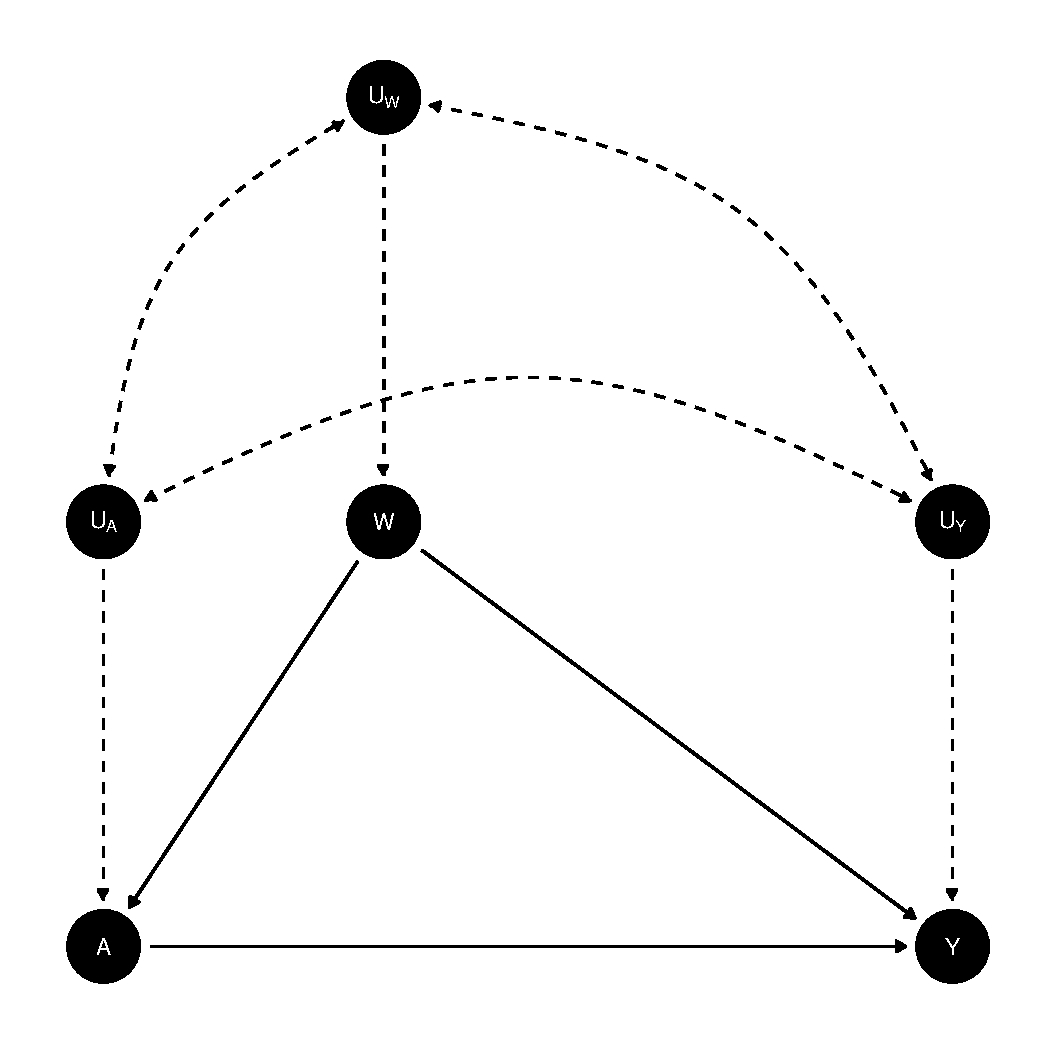
\includegraphics[width=4in]{figure/unnamed-chunk-2-1} 

\end{knitrout}

\end{figure}

\textbf{Does the SCM place any restrictions on $\mathcal{M}$?}

There are no independence assumptions, i.e., no restrictions on the distribution of the exogenous variables $\mathbb{P}_{\bm{U}}$. Nor are there any exclusion restrictions aside from the ordering of the recursive, time-ordered SCM.

  \end{enumerate}
    
  \item \textbf{Using the back-door criterion, assess identifiability of} $\Psi^F(P_{\bm{U},\bm{X}})$.
  
The back-door criterion states that for a set of covariates represented by the random variable $\bm{W}$, an exposure of interest represented by the random variable $A$, and an outcome of interest represented by the random variable $Y$, $\bm{W}$ satisfies the back-door criterion with respect to $A$ and $Y$ if $\bm{W}$ blocks any association between $A$ and $Y$ that arises from unmeasured common causes, does not create any new non-causal associations between $A$ and $Y$. and does not block any of the effect of $A$ on $Y$.

Another way to state the criteron graphically is that $\bm{W}$ satisfies the back-door criterion with respect to $(A,Y)$ if
  
  \begin{itemize}
    \item $\bm{W}$ blocks all paths from $A$ to $Y$ with an arrow into $A$, and
    \item No node in $\bm{W}$ is a descendant of $A$.
  \end{itemize}
  
If such a set $\bm{W}$ exists, then it meets the back-door criterion, which implies that the randomization assumption $Y_a \Perp \!\!\!\! A|\bm{W}$ holds, and thus we can identify the effect of $A$ on $Y$, specifically the target causal parameter $\Psi^F(P_{\bm{U},\bm{X}})$, as a parameter of the observed data distribution $\Psi(\mathbb{P}_{\bm{O}})$, by the G-computation formula:

\begin{align*}
\Psi^F(P_{\bm{U},\bm{X}}) = E_{\bm{U},\bm{X}}(Y_a)=\sum_{w}E_{\bm{O}}(Y|A=a,\bm{W}=\bm{w})P_{\bm{O}}(\bm{W}=\bm{w})=\Psi(\mathbb{P}_{\bm{O}})
\end{align*}
  
Unfortunately, in the SCM $\mathcal{M}^{F}$, $\Psi^F(P_{\bm{U},\bm{X}})$ is not identified as a parameter of $\Psi(\mathbb{P}_{\bm{O}})$, as the only measured variable available for satisfaction of the back-door criterion is $\bm{W}$ (or the empty set), and neither $\bm{W}$ nor the empty set meets the back-door criterion due to the remaining open back-door path between $A$ and $Y$ through $\bm{U_A}$ and $\bm{U_Y}$ (including the one through $\bm{U_A}$, $\bm{U_W}$, and $\bm{U_Y}$.)
  
  \begin{enumerate}[label=\textbf{(\alph*)}]
  
    \item \textbf{If not identified, under what assumptions would it be?}
    
The following DAGs show three possible working SCMs, $\mathcal{M}^{F^*}_1$, $\mathcal{M}^{F^*}_2$, and $\mathcal{M}^{F^*}_3$, that identify $\Psi^F(P_{\bm{U},\bm{X}})$, since $\bm{W}$ satisfies the back-door criterion as described above for all three. (All three assume that $\bm{U_A} \Perp \!\!\!\! \Perp \bm{U_Y}$, since if $\bm{U_A}$ and $\bm{U_Y}$ are associated, no means exists to block that path and thus satisfy the back-door criterion.)
    
\pagebreak
    
\begin{itemize}

  \item $\mathcal{M}^{F^*}_1$ assumptions (see Figure 2): 
  
  \begin{itemize} 
  
    \item $\bm{U_A} \Perp \!\!\!\! \Perp \bm{U_Y}$, i.e., the unmeasured factors $\bm{U_A}$ that influence energy expenditure $A$ do not affect and are not affected by the unmeasured factors $\bm{U_Y}$ influencing seven-year survival $Y$.
    
    \item $\bm{U_A} \Perp \!\!\!\! \Perp \bm{U_W}$, i.e., the unmeasured factors $\bm{U_A}$ that influence energy expenditure $A$ do not affect and are not affected by the unmeasured factors $\bm{U_W}$ influencing the smoking, body fat, and comorbidity covariates in $\bm{W}$.
    
  \end{itemize}
  
\begin{figure}

  \caption{Working structural causal model (SCM) $\mathcal{M}^{F^*}_1$ represented in directed acyclic graph (DAG) format.}
  \centering
    
\begin{knitrout}
\definecolor{shadecolor}{rgb}{0.969, 0.969, 0.969}\color{fgcolor}
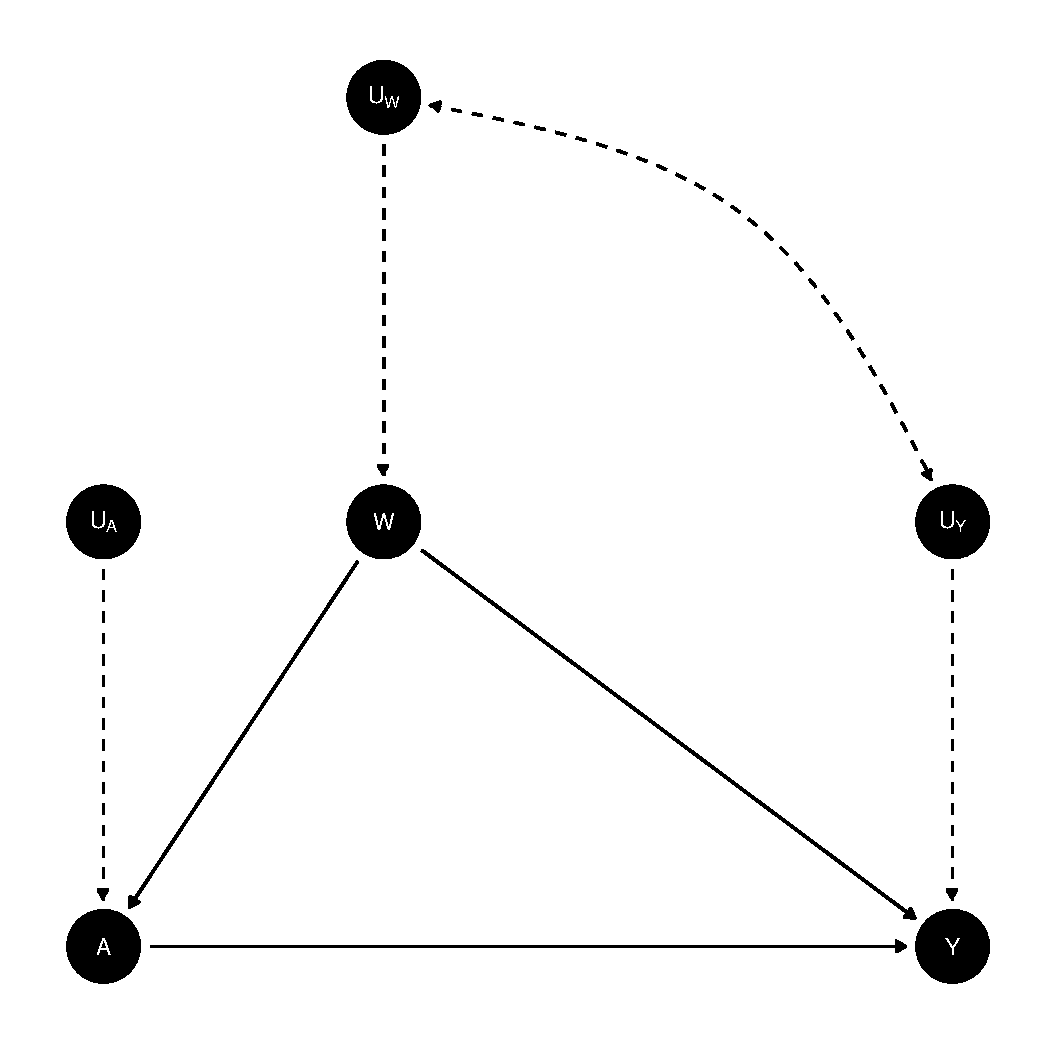
\includegraphics[width=4in]{figure/unnamed-chunk-3-1} 

\end{knitrout}

\end{figure}

\pagebreak

  \item $\mathcal{M}^{F^*}_2$ assumptions (see Figure 3): 
  
  \begin{itemize} 
  
    \item $\bm{U_A} \Perp \!\!\!\! \Perp \bm{U_Y}$ (as above).
    
    \item $\bm{U_W} \Perp \!\!\!\! \Perp \bm{U_Y}$, i.e., the unmeasured factors $\bm{U_W}$ that influence the smoking, body fat, and comorbidity covariates in $\bm{W}$ do not affect and are not affected by the unmeasured factors $\bm{U_Y}$ influencing seven-year survival $Y$.
    
  \end{itemize}
  
\begin{figure}
  \caption{Working structural causal model (SCM) $\mathcal{M}^{F^*}_2$ represented in directed acyclic graph (DAG) format.}
  \centering
  
\begin{knitrout}
\definecolor{shadecolor}{rgb}{0.969, 0.969, 0.969}\color{fgcolor}
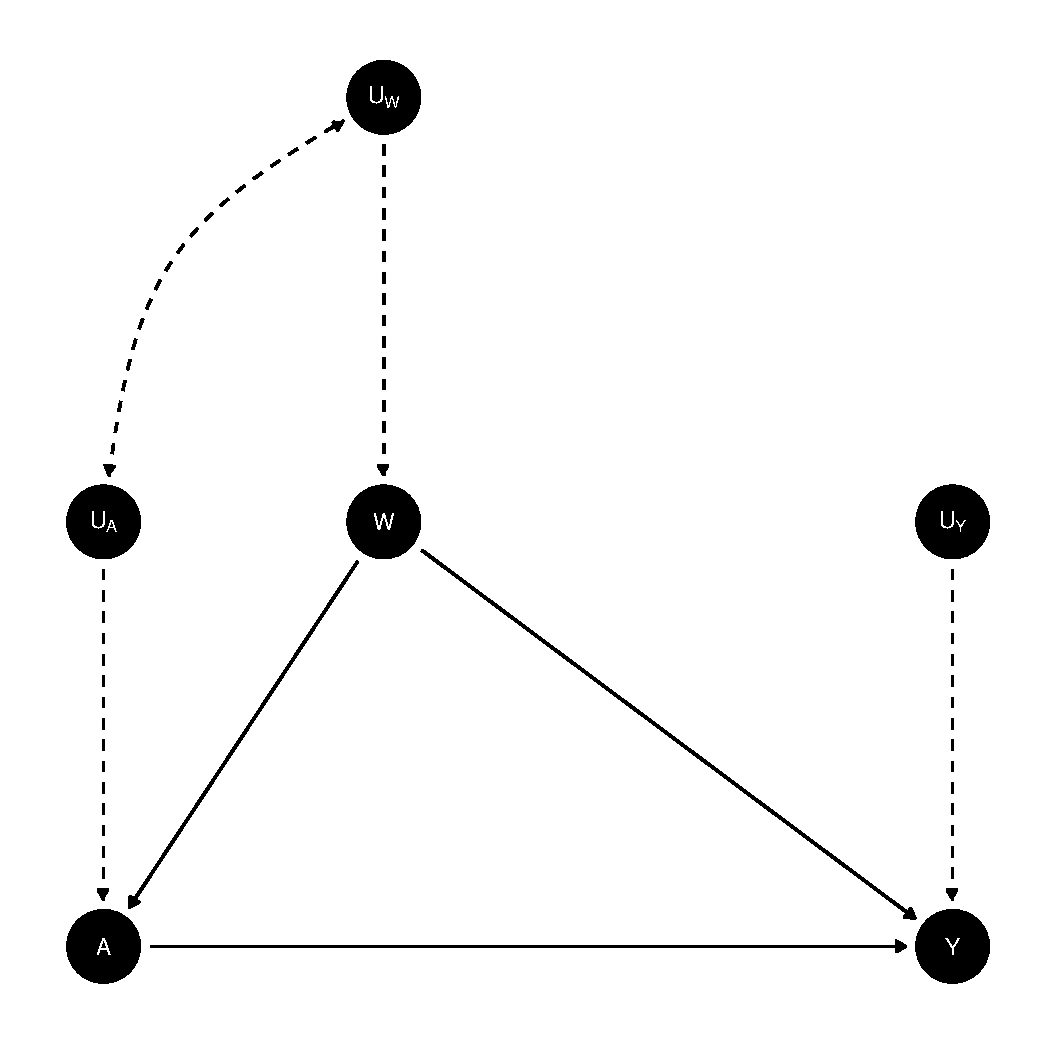
\includegraphics[width=4in]{figure/unnamed-chunk-4-1} 

\end{knitrout}

\end{figure}

\pagebreak

  \item $\mathcal{M}^{F^*}_3$ assumptions (see Figure 4): 
  
  All unmeasured factors are independent, i.e., 
  
  \begin{itemize} 
  
    \item $\bm{U_A} \Perp \!\!\!\! \Perp \bm{U_Y}$,
    
    \item $\bm{U_A} \Perp \!\!\!\! \Perp \bm{U_W}$, and
    
    \item $\bm{U_W} \Perp \!\!\!\! \Perp \bm{U_Y}$.
    
  \end{itemize}
  
\begin{figure}
  \caption{Working structural causal model (SCM) $\mathcal{M}^{F^*}_3$ represented in directed acyclic graph (DAG) format.}
  \centering
    
\begin{knitrout}
\definecolor{shadecolor}{rgb}{0.969, 0.969, 0.969}\color{fgcolor}
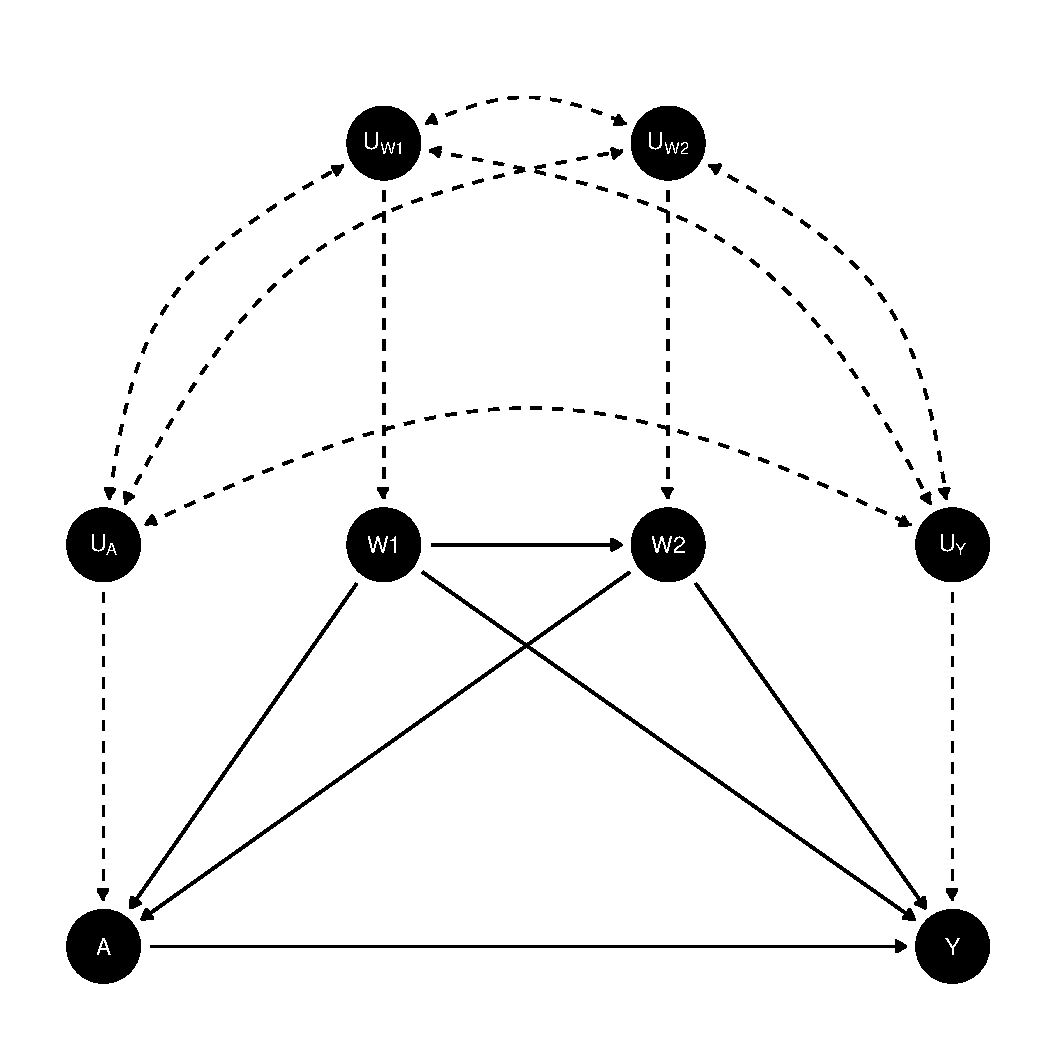
\includegraphics[width=4in]{figure/unnamed-chunk-5-1} 

\end{knitrout}

\end{figure}

\end{itemize}

\pagebreak
 
\textbf{Are some of these sets of additional assumptions more plausible than others?}

The fewer assumptions made, the more plausible the scenario, making working SCMs $\mathcal{M}^{F^*}_1$ and $\mathcal{M}^{F^*}_2$ more plausible than $\mathcal{M}^{F^*}_3$. 

All the working SCMs require the assumption that the unmeasured factors influencing energy expenditure be independent of the unmeasured factors influencing seven-year survival, i.e., that $\bm{U_A}$ be independent of $\bm{U_Y}$, or, alternately stated, that all factors influencing both $A$ and $Y$ be measured and included in $\bm{W}$. 

This assumption is likely not justified, as lots of unmeasured social and environmental factors likely influence both energy expenditure and survival but were not included in $\bm{W}$. Some examples:

\begin{itemize}

  \item Household wealth might also affect both energy expenditure, as a person with more might have more ability to join a gym, less need to work two jobs and more time for recreational exercise, etc., and survival due to access to a healthier diet, access to preventive healthcare, etc.; 
  \item Neighborhood gun violence could affect both energy expenditure, by reducing participant walking in the neighborhood, and all-cause seven-year survival directly, via exposure to bullets;
  \item Air pollution around a participant's home might make that participant less likely to exercise and also more likely to die from air pollution exposure;
  \item Social support might influence energy expenditure (e.g., by inspiring travel to meet friends) and is well documented as a factor that increases survival;
  \item Age or effects of aging, even witihin the range of ages in the study from 70 to 79, might affect both energy expenditure and seven-year survival.

\end{itemize}

That said, if a randomized controlled trial, for example, were to randomly assign participants into groups and then assign one group activities that increase energy expenditure and not the other, and were able to influence participants somehow not to alter their activities otherwise, that might make the assumption that $\bm{U_A}$ is independent of $\bm{U_Y}$ more plausible.

The working SCMs then also require at least one of two additional assumptions to achieve identifiability. $\mathcal{M}^{F^*}_1$ assumes that the unmeasured factors influencing the covariates listed above neither influence or are influenced by the unmeasured factors influencing the exposure of energy expenditure, i.e., that $\bm{U_W}$ is independent of $\bm{U_A}$.

This assumption is also likely not justified. Innumerable unmeasured factors likely affect both energy expenditure $A$ and the presence of various covariates in $\bm{W}$. Some examples:

\begin{itemize}
  \item An anxiety disorder might increase both energy expenditure and the incidence of various diseases included in $\bm{W}$;
  \item Household wealth might also affect both energy expenditure, as a person with more might have more ability to join a gym, less need to work two jobs and more time for recreational exercise, etc., and might also have a lower likelihood of the diseases in $\bm{W}$ due to access to a healthier diet, access to preventive healthcare, etc.; 
  \item Neighborhood gun violence could affect both energy expenditure, by reducing participant walking in the neighborhood, and the incidence of some of the diseases, behaviors, or comorbidities in $\bm{W}$ as ways to cope with or the effects of chronic stress;
  \item Air pollution around a participant's home might make that participant less likely to exercise and also more likely to develop some of the comorbidities in $\bm{W}$;
  \item Social support might influence energy expenditure (e.g., by inspiring travel to meet friends) and the incidence of some of the comorbidities in $\bm{W}$;
  \item Age or effects of aging, even given the limitation of the study to participants ages 70 to 79, might affect both energy expenditure and the incidence of some of the comorbidities in $\bm{W}$.
\end{itemize}

$\mathcal{M}^{F^*}_2$ assumes that the unmeasured factors influencing the covariates listed above neither influence or are influenced by the unmeasured factors influencing the outcome of seven-year survival, i.e., that $\bm{U_W}$ is independent of $\bm{U_Y}$.

This assumption is also likely not justified. Various factors likely affect both the values of the covariates in $\bm{W}$ and seven-year survival. Some examples:

\begin{itemize}
  \item A genetic mutation affecting cell repair might both affect cancer risk and might also affect all-cause seven-year mortality directly;
  \item Household wealth might also affect both the incidence of the comorbidities and smoking behavior in $\bm{W}$ as well as survival; 
  \item Neighborhood gun violence could affect both the incidence of some of the diseases, behaviors, or comorbidities in $\bm{W}$ as ways to cope with or the effects of chronic stress as well as survival directly via exposure to bullets;
  \item Air pollution around a participant's home might affect both the incidence of the comorbidities in $\bm{W}$ and survival via some other pathway not included in $\bm{W}$;
  \item Social support might influence both the incidence of some of the comorbidities in $\bm{W}$ and survival;
  \item Age or effects of aging, even given the limitation of the study to participants ages 70 to 79, might influence both the incidence of some of the comorbidities in $\bm{W}$ and survival.
\end{itemize}

\textbf{Are there additional measurements you could make so that the needed identifiability assumptions are more plausible?}

Additional measurements that would make the needed identifiability assumptions more plausible might be those evaluating the factors listed above, for the reasons given above. Factors that investigators could measure or data that they could collect via questionnaire include neighborhood of residence (which could be linked to area-level factors like air pollution exposure, gun violence rates, etc.), age, race/ethnicity, anxiety, perceived social support, household wealth, and (controversially) genetic sequencing.

In practice, I would probably use $\mathcal{M}^{F^*}_1$ as the working SCM (which assumes no association between $\bm{U_A}$ and $\bm{U_W}$ and no association between $\bm{U_A}$ and $\bm{U_Y}$). I would try to measure the factors listed in the prior paragraph and include them in $\bm{W}$ to make both of those assumptions more plausible. If nothing else, I would choose $\mathcal{M}^{F^*}_1$ because a truly randomized trial forces the independence of $U_A \Perp U_W$ and $U_A \Perp U_Y$, so a later researcher seeking to confirm conclusions from this observational study using a randomized trial to somehow assign energy expenditure could use a similar working SCM to confirm or challenging my results.

Moreover, should I gain access to additional data, I could check assumptions that $U_A \Perp U_W$ in my study data and possibly move factors from $\bm{U_W}$ to $\bm{W}$ much earlier and more easily than I could check assumptions that $U_W \Perp U_Y$ in my study data, as I would have access to the exposure data $A$ years before the outcome data $Y$. By the end of the study it might be too late to measure some of the factors in $\bm{U_W}$ that in my study turned out to be associated with the outcome $Y$.

Although I don't find any of these sets of assumptions particularly plausible, I also think that the assumption that $\mathcal{M}^{F^*}_1$ does not require, of no shared common causes between $\bm{U_W}$ and $\bm{U_Y}$, is perhaps the least plausible given the limited number of behaviors and comorbidities included in $\bm{U_W}$.
    
    \item \textbf{What notation do we use to denote the original SCM, augmented with additional assumptions needed for identifiability?}
    
    $\mathcal{M}^{F^*}$. Henceforth $\mathcal{M}^{F^*}$ refers to $\mathcal{M}^{F^*}_1$ above, which adds the following two assumptions:
    
    \begin{itemize}
      \item $\bm{U_W} \Perp \!\!\!\! \Perp \bm{U_A}$
      \item $\bm{U_A} \Perp \!\!\!\! \Perp \bm{U_Y}$
    \end{itemize}
    
  \end{enumerate}
  
  \item \textbf{Specify the target parameter of the observed data distribution (i.e., the statistical estimand).}
  
Under the working SCM $\mathcal{M}^{F^*}$, the target causal parameter of the observed data distribution, i.e., the statistical estimand, is 
  
\begin{align*}
\Psi(\mathbb{P}_{\bm{O}}) &= \mathbb{E}_{\bm{O}}[\mathbb{E}_O(Y|A=1,\bm{W}) - \mathbb{E}_{\bm{O}}(Y|A=0,\bm{W})] \\
&= \sum_{w}[\mathbb{E}_{\bm{O}}(Y|A=1,\bm{W}=\bm{w}) - \mathbb{E}_{\bm{O}}(Y|A=0,\bm{W}=\bm{w})]\mathbb{P}_{\bm{O}}(\bm{W}=\bm{w})
\end{align*}
  
  \item \textbf{What is the relevant positivity assumption? Are you concerned about violations of the positivity assumption in your study?}
  
The relevant positivity assumption is $\min_{a \in \mathcal{A}}P_O(A=a|\bm{W}=\bm{w})>0$ for all $\bm{W}$ for which $P_O(\bm{W}=\bm{w})>0$, i.e., that there must be a positive probability of each exposure level of $A$ within each possible stratum of covariate combinations in $\bm{W}$. Given the sheer number (12) of factors represented by $\bm{W}$, even without measuring the additional factors that I think are necessary to include in $\bm{W}$, and even if each factor in the existing $\bm{W}$ is binary, that leaves $2^{12}$ or 4,096 different possible combinations of covariate values in $\bm{W}$. Thus the assumption that each combination of covariate values actually present in $\bm{W}$ then exists for at least one treated and one untreated participant seems highly likely to be violated. Thus I am very concerned.

\end{enumerate}

\setlength{\leftskip}{0cm}

\section{Study-specific questions}

\setlength{\leftskip}{0.8cm}

\textbf{The investigators assume no unmeasured common causes of $(\bm{W}, A, Y)$. Is this necessary? Is this sufficient?} 

I'm not exactly sure if this is saying that the investigators made the weaker assumption that no single unmeasured cause caused all three, or that the investigators made the stronger assumption that none of the three share any unmeasured cause with another of the three, so I'll answer for both possibilities:

\vspace{2mm}

\textbf{The weaker assumption} that no single unmeasured cause exists that causes all three factors represented in the variable set $(\bm{W}, A, Y)$ is necessary but not sufficient. The case in which such an unmeasured cause does exist that affects all three is a subset of the scenario represented in the structural causal model of Figure 1, where all the unmeasured causes are associated with all other unmeasured causes. (Those associations could represent identity, i.e., that a single random variable representing the same cause is an element in all three random variables $\bm{U_W}$, $\bm{U_A}$, and $\bm{U_Y}$). The minimal situation, in which only one unmeasured cause $U$ exists but is a cause of $\bm{W}$, $A$, and $Y$, we can represent as in Figure 5.

\begin{figure}[H]
  \caption{Structural causal model where only one unmeasured cause $U$ exists but causes all three of $\bm{W}$, $A$, and $Y$.}
      
\begin{knitrout}
\definecolor{shadecolor}{rgb}{0.969, 0.969, 0.969}\color{fgcolor}
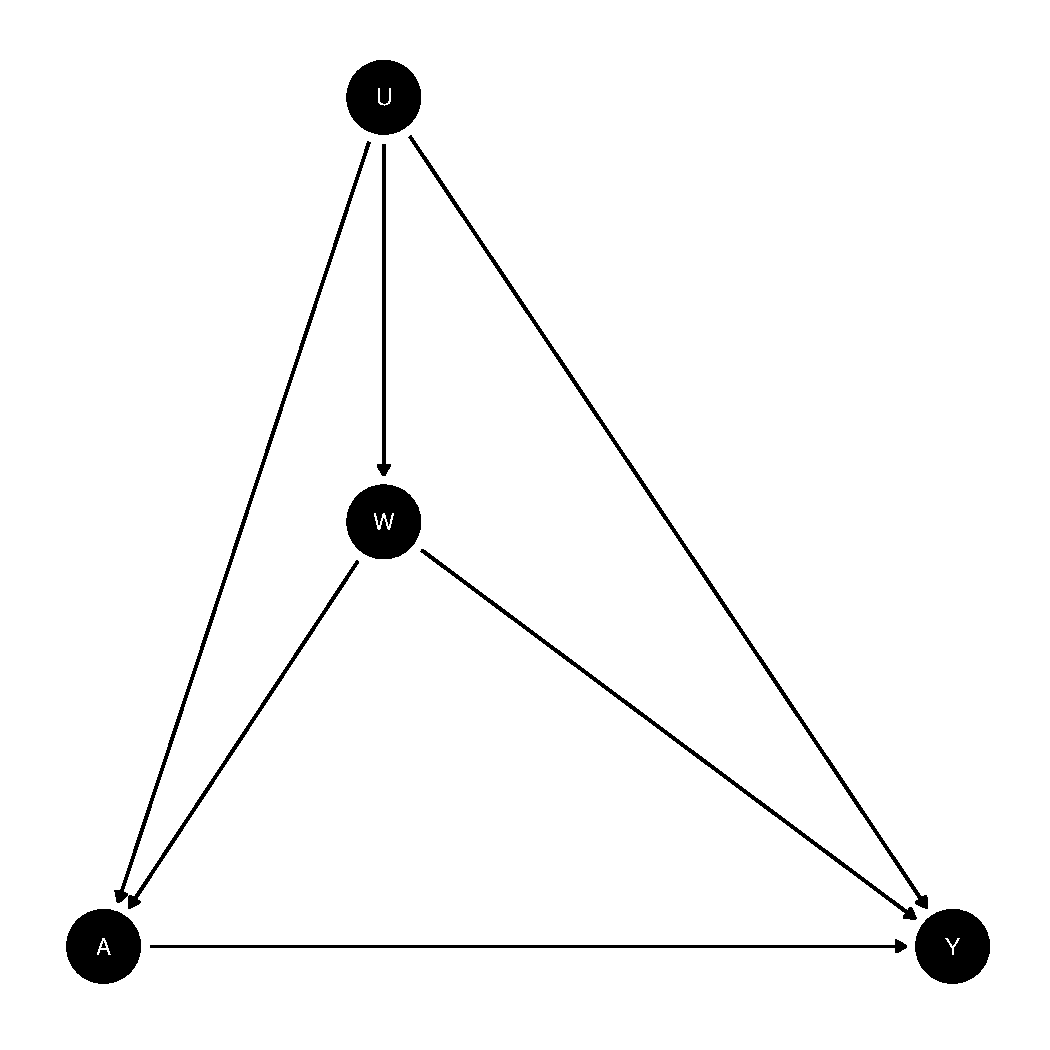
\includegraphics[width=4in]{figure/unnamed-chunk-6-1} 

\end{knitrout}

\end{figure}

Because $U$ is unmeasured, we cannot block the path through $U$ from $A$ to $Y$ by controlling for it, so we cannot satisfy the back-door criterion. Thus we cannot use the G-computation formula to identify the effect of energy expenditure $A$ on all-cause seven-year survival $Y$ with the data we have measured. We would need to measure the cause $U$ affecting all three. Thus, the assumption that no such $U$ exist is necessary. That said, though, the nonexistence of such a $U$ is not sufficient. Take the hypothetical case portrayed in Figure 6, where a common cause of $A$ and $Y$ exists that is not a cause of $\bm{W}$:

\begin{figure}[H]
  \caption{Structural causal model where only one unmeasured cause $U$ exists and causes $A$ and $Y$ but not $\bm{W}$.}
  \centering

\begin{knitrout}
\definecolor{shadecolor}{rgb}{0.969, 0.969, 0.969}\color{fgcolor}
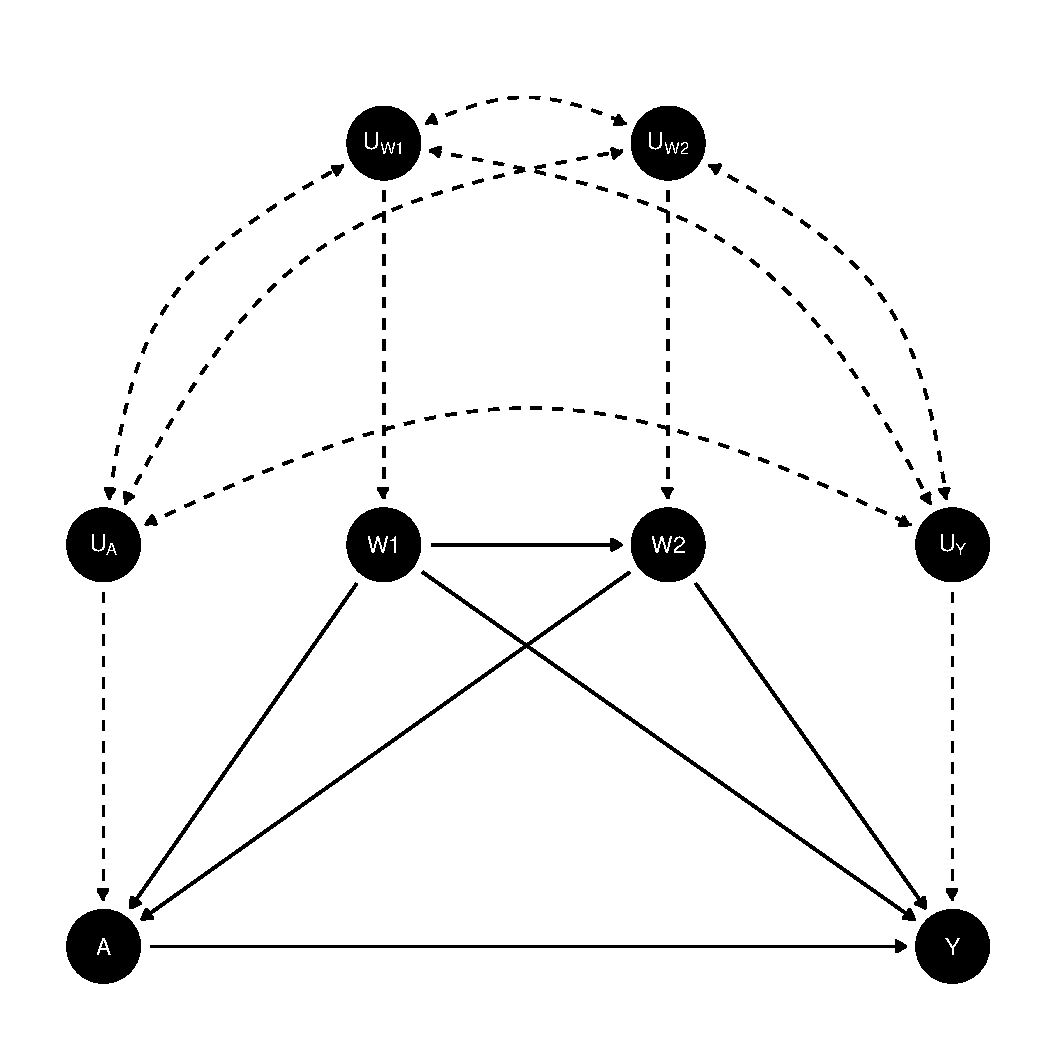
\includegraphics[width=4in]{figure/unnamed-chunk-7-1} 

\end{knitrout}

\end{figure}

Because $U$ is unmeasured, we cannot block the path through $U$ from $A$ to $Y$ by controlling for it, so we cannot satisfy the back-door criterion. Thus we cannot use the G-computation formula to identify the effect of energy expenditure $A$ on all-cause seven-year survival $Y$ with the data we have measured. We would need to measure the cause $U$ affecting both $A$ and $Y$. Thus, the assumption that no $U$ exists that affects all three of $\bm{W}$, $A$, and $Y$ is not sufficient to identify the target casual parameter as a parameter of the observed data distribution. We've shown by counterexample a situation in which no such $U$ exists but in which we still cannot satisfy the back-door criterion or use the G-computation formula to identify the effect of energy expenditure $A$ on all-cause seven-year survival $Y$ with the data we have measured.

\vspace{2mm}

\textbf{The stronger assumption} that none of the three factors represented in the variable set $(\bm{W}, A, Y)$ shares a common cause with another variable in the set is sufficient but not necessary. This case is represented by $\mathcal{M}^{F^*}_3$ in Figure 4. In this case, $\bm{W}$ blocks all paths with an arrow into $A$ without including any descendants of $A$, so it satisfies the back-door criterion, and we can use the G-computation formula to identify the target causal parameter $\Psi^F(P_{\bm{U},\bm{X}})$ as a parameter of the observed data distribution $\Psi(\mathbb{P}_{\bm{O}})$. Thus the assumption is sufficient.

The working SCMs $\mathcal{M}^{F^*}_1$ and $\mathcal{M}^{F^*}_2$ in figures 2 and 3, however, show that this assumption is not necessary, as the target causal parameter $\Psi^F(P_{\bm{U},\bm{X}})$ is also identifiable as a parameter of the observed data distribution $\Psi(\mathbb{P}_{\bm{O}})$ under those working SCMs despite the potential existence of a common cause of $\bm{W}$ and $Y$ in $\mathcal{M}^{F^*}_1$ (Figure 2) and the potential existence of a common cause of $\bm{W}$ and $A$ in $\mathcal{M}^{F^*}_2$ (Figure 3).

\vspace{2mm}

\setlength{\leftskip}{0cm}

\section{Questions for GSIs}

Hi, GSIs!

Maya's new slides for Lecture 5 appear to have a blank slide at the end labeled "Positivity for Continuous W" but no actual content on that slide. :(
      
\end{document} 
